\section{Recruitment Process Pipeline}

Figure~\ref{fig:tech-recruitment-pipeline} summarises a typical technical hiring pipeline.
Solid boxes denote core stages; dashed boxes are optional or organisation-dependent (more common in larger firms with the resources to run them).
The job offer is visually distinguished from intermediate stages.

\begin{figure}[htbp]
\centering
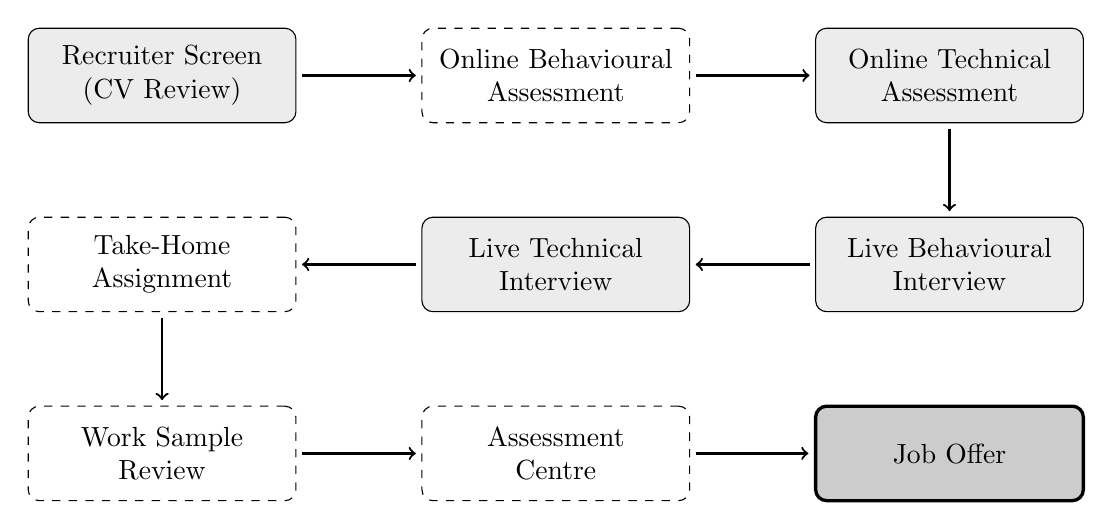
\begin{tikzpicture}[
    box/.style={
        draw,
        rectangle,
        rounded corners,
        align=center,
        minimum height=1.2cm,
        minimum width=3.4cm
    },
    core/.style={box, fill=gray!15},
    optional/.style={box, dashed},
    outcome/.style={
        box,
        fill=gray!40,
        draw=black,
        line width=1.2pt
    },
    arrow/.style={->, thick, shorten >=2pt, shorten <=2pt}
]

% ===== Row 1 =====
\node[core]     (cv)   at (0,0)   {Recruiter Screen\\(CV Review)};
\node[optional] (beh)  at (5,0)   {Online Behavioural\\Assessment};
\node[core]     (oa)   at (10,0)  {Online Technical\\Assessment};

% ===== Row 2 =====
\node[optional] (takehome) at (0,-2.4) {Take-Home\\Assignment};
\node[core] (techint) at (5,-2.4) {Live Technical\\Interview};
\node[core]     (live) at (10,-2.4) {Live Behavioural\\Interview};

% ===== Row 3 =====
\node[optional] (ac)    at (0,-4.8) {Work Sample\\Review};
\node[optional] (behint) at (5,-4.8) {Assessment\\Centre};
\node[outcome]  (offer) at (10,-4.8) {Job Offer};

% ===== Row 1 Arrows =====
\draw[arrow] (cv.east) -- (beh.west);
\draw[arrow] (beh.east) -- (oa.west);
\draw[arrow] (oa.south) -- (live.north);

% ===== Row 2 Arrows =====
\draw[arrow] (live.west) -- (techint.east);
\draw[arrow] (techint.west) -- (takehome.east);
\draw[arrow] (takehome.south) -- (ac.north);


% ===== Row 3 Arrows =====
\draw[arrow] (ac.east) -- (behint.west);
\draw[arrow] (behint.east) -- (offer.west);

\end{tikzpicture}
\caption[Technical recruitment pipeline]{Typical technical recruitment pipeline (core vs.\ optional stages).}
\label{fig:tech-recruitment-pipeline}
\end{figure}

When it comes to the application for technical positions, candidates will typically progress through multiple evaluation stages. 
While the sequence and steps taken often vary due to organisation size and maturity, industry research consistently shows that the technical recruitment pipelines will follow a multi-step structure \cite{cappelli2019}. 


\subsubsection{Recruiter Screen}
The hiring process for most organisations often starts off with a brief review of a candidate's CV to filter out 
candidates that are not suitable for the role. This is often performed by a recruiter or a hiring manager.
There has been a recent shift towards AI-driven pre-screening due to the rise in candidate applications, this
pre-screen is aimed to reduce the number of candidates that even make it to the first human review stage of the hiring process.
This significantly reduces applicant volumes, allowing for a more focused screening process, however, it is often at the cost
of algorithmic bias and opaque decision-making being introduced into the process.

Regardless of whether the process is a screen or a pre-screen, the CV itself is still the primary document evaluated.
However, industry research suggests that companies are becoming dissatisfied with typical CV data, such as past job titles
and educational prestige, when it comes to technical recruitment. It is noted that the industry is shifting towards skill-based
assessments to verify a candidate's competencies \cite{hackerrank2024skills}. Candidates are encouraged to provide their
GitHub URL as part of their application, however, research shows that this data is often reviewed inconsistently
during early stages, instead relying mainly on CVs as opposed to external behaviour evidence \cite{moore2023}.

\subsubsection{Online Behavioural Assessment} 
Larger enterprises commonly have an additional behavioural assessment, often in the form of a game, or a recorded interview, where candidates are prompted to record their response to common interview questions. 
Increasingly, these asynchronous video interviews are being augmented or fully driven by AI. Platforms employing machine learning 
algorithms can analyse a candidate's tone of voice, facial expressions, pacing, and keyword usage to algorithmically assess their 
personality and cultural fit. 
These tools, while uncommon in typical technical hiring pipelines, are more established in large-enterprise pre-screening: 
among Fortune 500 firms, 20\% already use asynchronous pre-recorded video interviews, with a further 17\% planning to adopt 
them, assessing dimensions such as communication style that are difficult to infer from a CV alone \cite{ithaka2018_assessment}. 
Smaller companies, however, rarely adopt such methods due to cost, limited perceived value and candidate-dropout risk.

\subsubsection{Online Technical Assessment}
Online technical assessments (commonly referred to as OAs) are core to the hiring process for many organisations. 
OAs often take place on platforms such as HackerRank and CodeSignal, and often focus on Data Structures and Algorithms (DSA). 
Industry surveys show that online technical assessments remain central to hiring pipelines: CoderPad's 2025 survey reports 
that 24.5\% of employers use asynchronous technical tests and 49.8\% use live coding interviews \cite{coderpad2025techhiring}, 
and CodeSignal highlights continued growth in standardised early-stage technical evaluations \cite{codesignal2023}.

\subsubsection{Live Behavioural Interview}
Live behavioural interviews are a common stage in technical recruitment, often conducted by HR or hiring managers to assess a candidate's cultural fit, communication skills and motivations for the role and company.
This process follows traditional interview formats, with a focus on behavioural questions alongside further discussions regarding the candidate's background, providing a better insight into a candidate's previous experiences and soft skills.

\subsubsection{Live Technical Interview}
Live technical interviews refer to the group of assessments which often involve an element of programming in front of an engineer at the hiring organisation, often involving live-coding, pair programming, or on-the-spot problem solving. 
These forms of assessment remain as a core part of the process for most software engineering hiring processes when it comes to evaluating a candidate's technical proficiency. 
As such, many organisations treat this as a central evaluation stage. 
While reliable aggregate data for this is scarce, multiple industry-level reports and practitioner accounts can confirm that live technical interviews remain an essential method for assessing candidates \cite{karat2020}. 

Some academic and industry critiques point out the limitations of this format, specifically stress under observation, lack of realism, and poor predictive validity for long-term developer performance. 
This suggests that hiring pipelines should leverage alternative assessment methods as opposed to solely live coding rounds \cite{behroozi2019hiring}.

\subsubsection{Take Home Assignment}
For organisations that prefer “skill-based hiring”, they may incorporate take-home tests as part of their technical hiring process. 
These assignments require a candidate to build or extend a small system, followed by a review interview. 
According to TestGorilla's 2024 survey, a large portion of employers report using assignment, or work-sample based assessments as a part of their hiring pipeline, highlighting the relevance of take-home assessments for a realistic evaluation of coding ability and design choices \cite{testgorilla2024}. 
They argue that these assignments provide a better benchmark for the candidate's real-world development skills rather than time-limited algorithmic tests and whiteboard interviews.

\subsubsection{Work Sample Review}
Many employers like to also use real-world evidence, such as GitHub repositories, open-source commits and portfolio projects to assess a candidate's ability to build software. 
This data is often a critical differentiator, as it is able to separate a candidate's claims from their actual abilities.
Historical data highlight that the majority of firms (80\% of small and 66\% of large firms) place high value on portfolio evidence,
such as GitHub \cite{hackerrank2018skills}. Recent reports also come to a similar conclusion, that verified technical 
assessments are essential in addressing the limitations of traditional CVs \cite{hackerrank2024skills}.
However, this is often done later in the pipeline due to the time and expertise required for evaluation. 
Academic literature shows that work-sample tests are one of the highest-validity predictors of job performance (validity coefficient of 0.54) \cite{schmidt1998}, significantly outperforming CV-based assessments.

\subsubsection{Assessment Centre}
An assessment centre (commonly referred to as AC) is a structured multi-exercise evaluation process, often used in graduate programs and enterprise-level hiring. 
Recent UK survey data suggest that a minority of organisations (32\% in 2020) use formal assessment centres as part of their selection process \cite{cipd2020_resourcing}. 
Where assessment centres are used, UK employers commonly apply methods such as group exercises, psychometric tests, role plays and combined tasks to evaluate teamwork, communication and problem-solving \cite{cipd2022}. 
While not widely used, ACs remain useful for gaining deeper insights into the candidate's interpersonal and non-technical capabilities.

\subsubsection{Relevance to MERIT}
Given the complexities and inconsistencies that are present in the technical hiring process, the screening stage remains to be the most influential, yet error prone point in the process. 
Organisations rely heavily on this filter, yet early decisions are often solely based on a brief CV review, which is often shown to be vulnerable to bias, information loss and unreliable judgement. 
MERIT will target this part of the pipeline to improve accuracy, fairness and evidence-quality in order to produce the greatest organisational impact.

MERIT will strengthen screening through the integration of multi-source evidence, such as GitHub activity, CV data, and other sources, to provide verifiable behavioural and technical indicators. 
This early-stage assessment can reduce or refine the need for later steps, such as online coding tests, manual work-sample reviews, and broad behavioural screens, while still highlighting areas where further evaluation is necessary. 
The system will be designed to be adaptable across different organisation sizes, for example smaller firms will benefit from reduced reliance on time-consuming take-home tasks, and larger firms can improve their structured assessments with transparent data-driven insights. 
By transforming the earliest decision point into a more reliable and insightful stage, MERIT helps to create a fairer, more consistent and efficient technical hiring process.
